\documentclass[aip,pop,numerical,reprint,floatfix]{revtex4-1}
\usepackage[T1]{fontenc}
\usepackage[latin9]{inputenc}
\usepackage{array}
\usepackage{rotating}
\usepackage{verbatim}
\usepackage{graphicx,epstopdf}
\usepackage{setspace}

\makeatletter

%%%%%%%%%%%%%%%%%%%%%%%%%%%%%% LyX specific LaTeX commands.
%% Because html converters don't know tabularnewline
\providecommand{\tabularnewline}{\\}

\makeatother

\begin{document}

\title{Three-dimensional simulations of NIF implosions: insight into experimental
observables}

\author{Brian K. Spears}
\email{spears9@llnl.gov}
\author{David H. Munro}
\author{Scott Sepke}
\author{Joseph Caggiano}
\author{Dan Clark}
\author{Robert Hatarik}
\author{Andrea Kritcher}
\author{Dan Sayre}
\author{Charles Yeamans}
\affiliation{Lawrence Livermore National Laboratory, P.O. Box 808, Livermore, California 94551-0808, USA}

\author{Jim Knauer}
\affiliation{Laboratory for Laser Energetics, 250 E. River Road Rochester, New York 14623-1212, USA}

\author{Terry Hilsabeck}
\author{Joe Kilkenny}
\affiliation{General Atomics, P.O. Box 85608, San Diego, California 92186-5608, USA}

\begin{abstract}
We simulate in 3D both the hydrodynamics and, simultaneously, the
X-ray and neutron diagnostic signatures of National Ignition Facility
(NIF) implosions. We apply asymmetric radiation drive to study the
impact of low mode asymmetry on diagnostic observables. We examine
X-ray and neutron images as well as neutron spectra for these perturbed
implosions. The X-ray images show hot spot evolution on small length
scales and short time scales, reflecting the incomplete stagnation
seen in the simulation. The neutron images show surprising differences
from the X-ray images. The neutron spectra provide additional measures
of implosion asymmetry. Flow in the hot spot alters the neutron spectral
peak, namely the peak location and width. The changes in the width
lead to a variation in the apparent temperature with viewing angle
that signal underlying hot spot asymmetry. We compare our new expectations
based on the simulated data with NIF data. We find that some recent
cryogenic layered experiments show appreciable temperature anisotropy
indicating residual flow in the hot spot. We also find some trends
in the data that are at odds with our simulation and theoretical understanding.
\end{abstract}

\maketitle

\section{\label{sec:Introduction}Introduction}

Implosion experiments in the inertial confinement fusion (ICF) program
at the National Ignition Facility (NIF) aim to produce thermonuclear
fusion by assembling a spherically symmetric hot spot surrounded by
cold, dense deuterium-tritium (DT) fuel \cite{edwards_nif_progress_2012}.
Experiments to develop an igniting platform have entered the alpha-heating
regime by producing more than twice as much neutron yield as an equivalent
implosion not self-heated by alpha particles \cite{hurricane_nature,hurricane_nature_corrigendum}.
However, the current performance is likely limited by asymmetry in
the implosion leading to incomplete stagnation and residual flow in
the hot spot throughout the fusion burn process. 

Here we investigate the experimental signatures of implosion asymmetry.
We do this by simulating in 3D an ICF experiment. The simulation includes
detailed radiation transport and hydronamics done by HYDRA \cite{marinak_hydra_2001}. In addition,
we simulate a large set of diagnostics and the experimental signatures
they record -- X-ray images, neutron images, and neutron spectra,
among others. 

We find that shape distortions in the implosion may be seen differently
by X-ray and neutron cameras. Furthermore, X-ray images themselves
may appear very similar across observed X-ray energy bands. Our simulated
neutron spectra show angular dependence of neutron peak centroid shift
and neutron peak width as predicted by recent theoretical work \cite{appelbe_relativ_2014,murphy_neut_spectrum}.
The fluid velocity distribution in a non-stagnated implosion increases
the neutron peak width, which may be misinterpreted as an increase
in ion temperature \cite{brysk_tion_1973}. We point out that variation
with viewing angle of the neutron peak width, caused by angular variation
in the fluid velocity, is a nuclear-based measure of implosion asymmetry
complementary to X-ray imaging.

Equipped with expectations based on our simulated diagnostics, we
turn to the database of results from recent high-foot implosions on
NIF for comparison. The examination reveals that nuclear signatures
of asymmetry are present in the NIF database. These asymmetries range
from very small to quite substantial. In the most asymmetric cases,
we find a correspondence between X-ray image distortion and nuclear
asymmetry signatures. We also find some trends that are not consistent
with simulation-based expectations. Here we point to the angular variation
of neutron peak width as seen in both DT and DD neutrons where the
relationship between the two signatures differs in experiment from
that seen in 3D simulation. 

\section{\label{sec:3d_sims}Simulation of 3D implosions with low-mode asymmetry }


\subsection{\label{sec:numerical}Numerical methodology}

We begin our investigation of asymmetries with 3D radhydro simulations
of a high foot implosion \cite{dittrich_highfoot_prl}. These high adiabat implosions
show low instability growth at the ablation front. Thus perturbations
communicated to the hot spot by low-mode-asymmetric radiation drive
dominate. The ICF program has focused in the past on correcting small
drive perturbations based on detailed 2D modeling \cite{landen_tuning}. However, experimental X-ray images from NIF
implosions show that hot spot shape, inferred from x-ray self-emission
\cite{kyrala_nif_symmetry_2010}, are neither spherical nor axisymmetric \cite{peterson_lpi_3d}.
Decomposing the hot spot into spherical harmonics ($Y_{lm}$), we
find contributions for $l,m\leq4$. Consequently, we focus on simulations
supporting asymmetric perturbations with this frequency content.

Our radhydro simulation proceeds in two phases. First, we initiate
the problem on a spherical polar mesh and define the asymmetric radiation
drive. The radiation flux driving the capsule has angular asymmetry
described by a spectrum of $l$ and $m$ numbers. The magnitude of
the components is also time-dependent. In particular we chose to apply
dynamically varying $Y_{2,0}$ and $Y_{4,0}$ consistent with post-shot
investigations of high-foot experiments \cite{kritcher_dynamic_p2p4}. To make the radiation asymmetry fully 3D, we apply
a mode 1 perturbation, $Y_{1,-1}=Y_{1,0}=Y_{1,1}=0.03*Y_{0,0}$ exclusively
in the high-flux peak of the radiation drive. Previous work \cite{spears_mode1_pop_140409}
shows that this type of perturbation produces asymmetry in both X-ray
and nuclear diagnostic signatures at clearly detectable levels. To
resolve asymmetries of these wavelengths in the early implosion phase,
from the initial shell radius of about $1000$ $\mu m$ to an imploded
shell radius of about $250$ $\mu m$, we require only modest angular
resolution of 128 mesh lines in both angular directions. This is substantially
lower resolution than the extremely detailed simulations described
by Clark et al. \cite{clark_detailed_postshot_pop2012}. This lower
resolution frees up computational resources, the most precious of
which is system memory, to do detailed Monte Carlo simulations of
thermonuclear burn processes, discussed in more detail later.

Once the dense shell has imploded to $250$ $\mu m$, the asymmetric
radiation drive produces high-speed flows through the nascent central
hot spot. The singular origin in the spherical polar mesh and the
large aspect ratio zones surrounding it poorly resolve the lateral
flows in the imploded core. This motivates us to remap the problem
to a multi-block box mesh. This mesh replaces the
singular origin point with a logically Cartesian box. Additional blocks
are connected to the central box faces and to each other, producing
7 connected boxes that cover the problem. The remap not only produces
a topology that better handles the flow, but also allows high resolution
to be focused on the forming hot spot where we resolve flows on the
$10$-$\mu m$ length scale. The simulation runs through stagnation,
peak neutron production, and later decompression on this mesh topology.

\subsection{\label{sec:implosion}Description of the implosion}

The 3D asymmetric radiation drive produces strong flows that disrupt
and perturb the hot spot. The 1 keV isosurface can be thought of as
the boundary of this hot spot. In Figure \ref{fig:3d_hist}, we show the
evolution of the hot spot boundary from t=-100ps to peak neutron production
at t=0ps. The hohlraum axis is vertical here. In frames (a) - (c),
the mode 2 and mode 4 dynamic asymmetry has produced oscillations
in the hot spot boundary at modes 2 and 4. Namely, the hot spot is
swinging from prolate back through spherical, and similarly for mode
4. The mode 1 asymmetry results in a radiation drive imbalance --
high drive at the top right and low drive at the bottom left. This
imbalance produces a mode-1-induced jet \cite{spears_mode1_pop_140409}
forming in (c), but evolving until it has crossed the entire hot spot
by bang time in (f). This jet feature is a hallmark to be tracked
in later analysis of the simulated diagnostics.

\begin{figure*}[htb]
\centering
\includegraphics[width=0.8\paperwidth]{turkey_hist}
\caption{\label{fig:3d_hist}cut-away of simulated hot spot boundary.  We take the 1 keV ion temperature isosurface as the hot spot boundary.  We have shown it here at several times approaching peak neutron production. The hot spot evolves from 100 ps before peak neutron production (panel (a)) until the time of peak production (panel (f)). The time-dependent asymmetry produces oscillations in the hot spot shape and drives a strong jet that penetrates the hot spot from the top right.}
\end{figure*}

We find additional insight by examining the hot spot from a variety
of angles at a fixed time, neutron bang time, in Figure \ref{fig:3d_spin}.
There are two features of primary interest. First, the mode-1 jet
has fully penetrated the hot spot, leaving a substantial hole, most
visible in frames (b), (c), or (d). We will show in Sec. \ref{sec:sim_diagnostics}
that such a 3D feature is visible in X-ray images only with high resolution.
The second feature of interest is the higher-mode content in the hot
spot shape. Flows on the 10-$\mu m$ length scale develop throughout
the stagnation phase and are seeded wholly by the low-mode drive perturbation.

\begin{figure*}[htb]
\begin{centering}
\includegraphics[width=0.8\paperwidth]{turkey_spin}
\par\end{centering}
\caption{\label{fig:3d_spin}hot spot viewed from different angles. We show here the hot spot boundary (1 keV isosurface) at peak neutron production. The panels show the hot spot as viewed from multiple directions. We note the small scale length structure that develops and also highlight the hole that has been punched in the hot spot by the jetl}
\end{figure*}

%FINISH THIS ----------------------------------------------------------------------------
This degradation of the hot spot has substantial impact on implosion
performance \cite{spears_metrics_pop_invited_2012}. Table \ref{tab:1d_3d_performance}(comparison
of 1D, 3D performance plus table). note in 3D: reduced yield/pressure,
reduced Tion, increased apparent Tion (see diags later), early bang
time.
%FINISH THIS ----------------------------------------------------------------------------

\begin{table}[h]
\begin{centering}
\begin{tabular}{|l|c|c|}
\hline 
 & 1D & 3D\tabularnewline
\hline 
\hline 
Yield {[}neutrons{]} & 1.1e15 & 3.3e14\tabularnewline
\hline 
Average Thermal $T_{ion}$ {[}keV{]} & 2.4 & 2.2\tabularnewline
\hline 
Apparent $T_{ion}$ {[}keV{]} & 2.4 & 3.2\tabularnewline
\hline 
Bang time {[}ns{]} & 16.64 & 16.54\tabularnewline
\hline 
Peak pressure {[}Gbar{]} & 173 & 60\tabularnewline
\hline 
\end{tabular}
\par\end{centering}
\caption{\label{tab:1d_3d_performance}}
\end{table}

\section{\label{sec:sim_diagnostics}Detailed simulated diagnostic output}

We put special emphasis on simulating in detail the diagnostic signatures
measured by NIF instruments. These signatures, produced by both neutrons
and x-rays, provide our view into the experimental implosions. Ultimately,
our understanding of the experiment rests on our expectations about
these signatures. Our principal goal is to better understand the effects
that large, 3D asymmetries have on the diagnostic observables and
what these signatures can tell us about the asymmetry and quality
of our implosion. We have arrived at some new expectations and hypotheses
about data based on our diagnostic simulations, and we describe those
here.

For the first time, we can simultaneously simulate low-resolution
hydrodynamics and detailed neutron and X-ray production in three dimensions.
We discuss Monte Carlo neutronics first, where managing computational
resources is critical. HYDRA transports neutrons, gamma rays, and
light ions (hydrogen and helium isotopes) produced during burn. We
account for elastic and inelastic collisions, including in-flight
reactions of daughter particles, Doppler shifts, and relativistic
kinematics. Charged particles, in particular alpha particles, slow
down and heat the simulated plasma, including recoils from neutron
collisions. We tally important quantities to build simulated diagnostics.
For example, when a neutron escapes the simulation, we tally its speed
and direction to build the energy spectrum of escaping neutrons. 

However, too few of these transport Monte Carlo particles happen to
escape in the direction of some diagnostic instrument (such as a neutron
imager or neutron time-of-flight spectrometer), to build an image
or spectrum accurate enough to compare to real data. Hence, along
a few specific lines of sight, we track a population of diagnostic
neutrons (for example), all moving in a single direction toward some
detector, which do not contribute back to the hydrodynamic simulation
like the transport particles. These diagnostic particles solve the
adjoint problem \cite{duderstadt_book}, and therefore need not be fully
tracked like the transport particles. Each nuclear event (e.g.- TN
reaction or collision) among the transport particles launches some
number of diagnostic neutrons directly toward the desired detector,
carrying a weight equal to the number of neutrons per steradian moving
in that direction, and with energy according to the distribution,
the event would produce. We track this diagnostic neutron along its
straight line path, decrementing its weight by the probability that
it would scatter or be absorbed by further Monte Carlo nuclear events
as it flies out of the plasma, then tally the number of neutrons per
steradian it represents on exit, along with its energy and trajectory.
Since their weight is infinitesimal (neutrons per steradian), diagnostic
neutrons have no effect on the plasma and produce no additional Monte
Carlo particles to track. Despite the huge improvement in statistics
for building a diagnostic signal, we still consume all of the memory
on our computer, 16{*}64 GB of RAM, to hold these diagnostic particles
together with the transport particles and plasma simulation. 

We transport X-rays by multigroup diffusion in the HYDRA simulation,
since Monte Carlo radiation transport would be too expensive. But
we simulate X-ray images by straightforward three dimensional ray
tracing: To simulate a given camera, we construct a square grid of
parallel rays, one ray per image pixel, each ray directed toward the
diagnostic. The 300 um/ps speed of X-rays is practically infinite,
and at core imaging energies, X-ray refraction is negligible. Thus
at each instant of time, we simply integrate the transport equation
on each ray as it passes through the hexahedral HYDRA mesh. For the
ray trace, we augment the LTE absorption opacity we use for transport
by the (Thompson) scattering proportional to the free electron density.
We augment the LTE emissivity by a corresponding amount proportional
to both electron density and radiation density, so that the augmented
opacity accounts for scattering out of the ray, while the augmented
emissivity accounts for scattering into the ray. This in-scatter is
isotropic, consistent with the diffusive radiation transport, with
similar failure to represent the directionality of the radiation field.
For each ray, we compute the sequence of cells and the length of the
ray segment inside each cell. Assuming each cell is a uniform emitter
and absorber with its augmented emissivity and opacity, we compute
the attenuation and self-emission produced by each segment. Finally,
we accumulate the self-emission, that is, power per unit area per
steradian in each photon energy group, with each cell in the sequence
attenuating what enters and contributing its own self-emission. The
total emission from the final cell in the sequence is the contribution
of that ray to the image at that time. We sum over photon energy and
integrate over time according to the spectral response and temporal
gating function, respectively, of the instrument we are simulating
in order to produce a final image.

\subsection{\label{sec:sim_xray_neut}Simulated X-ray and neutron images}

We now examine simulated X-ray image sequences (movies) to better
understand the detailed evolution of the hot spot. We show in Figure \ref{fig:dixi-image}
the 9 keV x-ray emission at multiple spatial resolutions and several
times before and at peak neutron production. The images show several
key features. First, the mode-1 induced jet visibly dims the hot spot
during its transit (compare Figure \ref{fig:3d_hist} panel (e) and Figure \ref{fig:dixi-image}
at -90 ps. This feature is a hallmark of the mode-1 radiation imbalance
responsible for much of the degradation from 1D performance. Yet,
it requires at least 10 $\mu m$ resolution to identify this feature
in the images. Also notable is the short-scale-length structure visible
in the 1-$\mu m$ resolution images. Similar structure was noted in
Figure \ref{fig:3d_spin}. In the x-ray images, emission from Si-doped CH
ablator material mixed in the initial DT gas emphasizes these fine-scale
flows. Again, this structure is lost by 20-$\mu m$ resolution. We
finally highlight dynamic evolution across frames. The time-dependent
drive asymmetry has produced hot spot flows that evolve substantially
on the 30-ps time scale. These observations from simulated images
suggest that we should expect rapid, fine scale evolution in x-ray
self emission images, and they have supported the development of a
high-performance x-ray camera capable of 10 $\mu m$ spatial and 10
ps temporal resolution. This camera, known as DIXI, has been successfully
deployed on NIF experiments beginning with a DT-layered implosion
N140819. The data confirm dynamic evolution with characteristic scales
similar to those reported here {[}cite Sabrina{]}. 

\begin{figure*}[h]
\begin{centering}
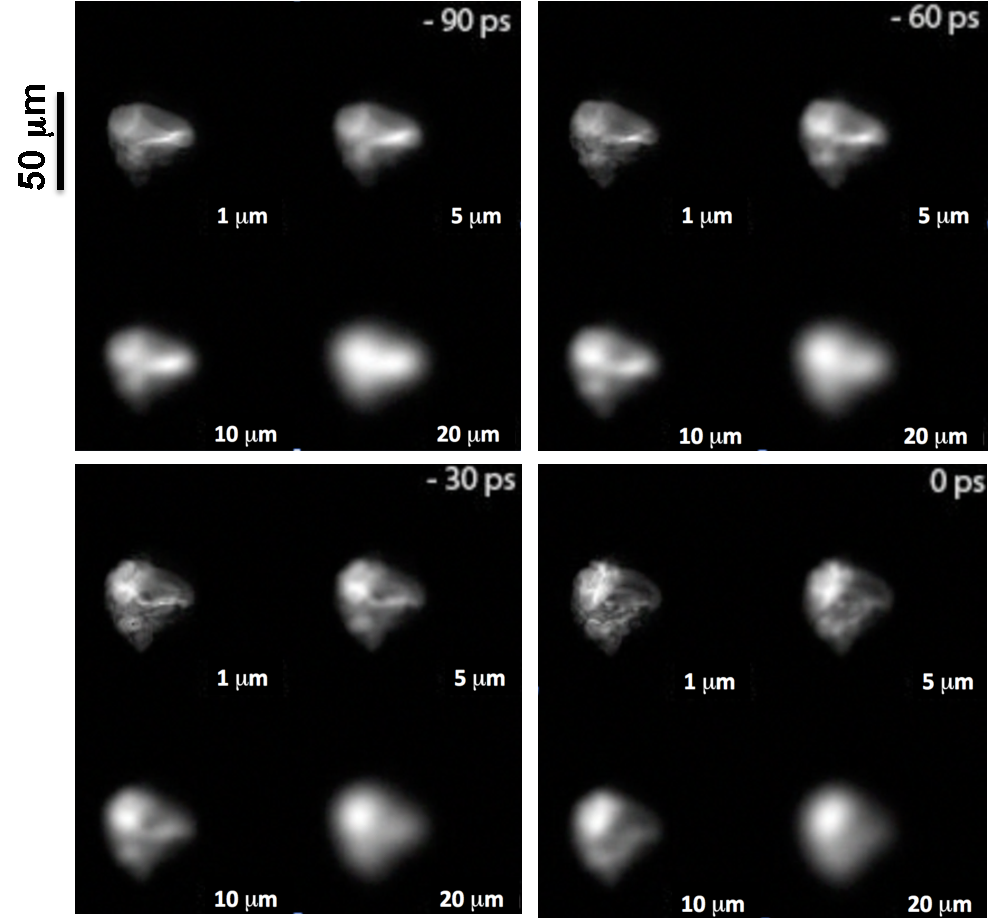
\includegraphics[width=0.8\paperwidth]{dixi_sim}
\par\end{centering}
\caption{\label{fig:dixi-image}simulated X-ray images with high temporal and spatial resolution.  We show simulated 9 keV X-ray images at four times: -90 ps, -60 ps, -30 ps and 0 ps, where 0 ps is the time of peak neutron yield. Each time shows four resolutions: 1 $\mu m$,  5 $\mu m$, 10 $\mu m$, and 20 $\mu m$. The fine scale features, jet, and rapid evolution discussed in figures Figure \ref{fig:3d_hist} and Figure \ref{fig:3d_spin} are clearly visible at 1 $\mu m$ resolution. By 20 $\mu m$, the features are difficult to identify. }
\end{figure*}

We have also compared x-ray images filtered for a variety of x-ray
energy bands, namely 9, 12, 16, and 20 keV (see Figure \ref{fig:multi-energy_xray}).
To our surprise, the image topography is very similar. Conventional
expectations suggest that the relatively stronger attenuation of 9
keV x-rays by cool CH ablator material would alter the hot spot emission
images. Higher-energy 20 keV x-rays would be expected to more effectively
escape the ablator, emphasizing the hottest parts of the hot spot.
In fact, the brightness of the images is reduced with energy as expected.
However, image shapes are nearly unchanged across energies. Thus,
the ablator material, in the simulations, effectively acts as an intensity
filter without affecting spatial gradients across energies.

\begin{figure}[htb]
\begin{centering}
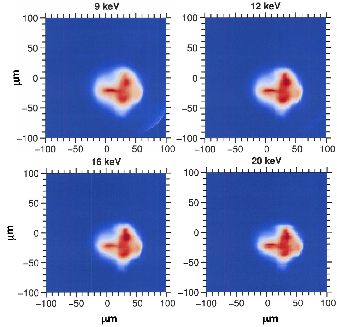
\includegraphics[width=0.8\columnwidth]{multi-energy_xray}
\par\end{centering}
\caption{\label{fig:multi-energy_xray}X-ray images at multiple energies. Simulated X-ray images at 9 keV, 12 keV, 16 keV, and 20 keV show little difference in appearance across energies, though the total signal falls as expected.}
\end{figure}

We find additional insight by comparing x-ray images to primary neutron
images in Figure \ref{fig:xray_vs_neuts}. The primary neutron images are
filtered to accept mostly unscattered neutrons from a 13 to 15 MeV
band centered at the (approximately) 14 MeV DT neutron birth energy.
Thus the primary neutron images provide an alternative view of the
hot spot. Again, conventional expectations are that the x-ray and
neutron images reflect process that scale in grossly the same way
with temperature and density. Consequently, they might be expected
to be very similar. However, we find key differences in the images.
Though the physics of the image production is complicated, we believe
two mechanisms are the chief sources of the the discrepancies. First,
the emissivity of neutrons increases less strongly with temperature
than does the emissivity of x-rays. This drives x-rays to emphasize
temperature gradients more strongly than do neutrons. Differences
in temperature histories of both electrons and ions are also a source
of discrepancy. The X-ray production peaks more than 50 ps before
the neutron production. During the first half of the x-ray production,
the ion temperature, which drives neutron production, is higher than
the electron temperature, which drives x-ray production. This means
that X-ray and neutron signals are weighting different times of the
implosions as well. Together, the dissimilar emissivities and histories
mean that the two production processes can emphasize different times
and spatial locations in the hot spot. Viewed this way, it is less
surprising that the lobed neutron image in Figure \ref{fig:xray_vs_neuts}
displays a bright bottom left lobe and a dim top right lobe compared
to the more uniform X-ray image. Nevertheless, it is exceedingly difficult
to probe the 3D simulation in space and time to determine the exact
physical sequencing and sensitivities that lead to the particular
image differences shown. 

\begin{figure}[h]
\begin{centering}
\includegraphics[width=0.8\columnwidth]{xray_vs_neut}
\par\end{centering}
\caption{\label{fig:xray_vs_neuts}hard X-ray and primary neutron images. Time-integrated X-ray and neutron images are different. Differences in temperature sensitivity of emissivity for the X-rays and neutrons provide a partial explanation. Differences in electron and ion temperature histories also lead to disparities.}
\end{figure}

\subsection{\label{sec:sim_spectra}Simulated neutron spectra}

Neutron spectra, as compared to images, are amenable to very detailed
analysis coupling the fluid state, thermodynamics and fluid dynamics,
with the neutron production. Analysis of the spectra gives multiple
features that reflect the state of the emitting plasma. These include
the location (in neutron energy or neutron velocity) of the primary
peak of the spectrum and the width of this peak (see Figure \ref{fig:neut_spectrum}).
Detailed theory shows that these features encode the hot spot's thermal
temperature, its bulk translation, and its internal, residual flow.

The spectra are measured in experiments by neutron time-of-flight
(nTOF) detectors \cite{glebov_ntof_NIF_test}.
As neutrons propagate from the hot spot to the nTOF located about
20 m away, the neutrons disperse based on energy -- the most energetic
particles arriving before those with less energy. The spectral resolution
results from the temporal resolution of arrival time at the detector.
\begin{comment}
peak shift, bulk velocity.
\end{comment}

\begin{figure}[h]
\begin{centering}
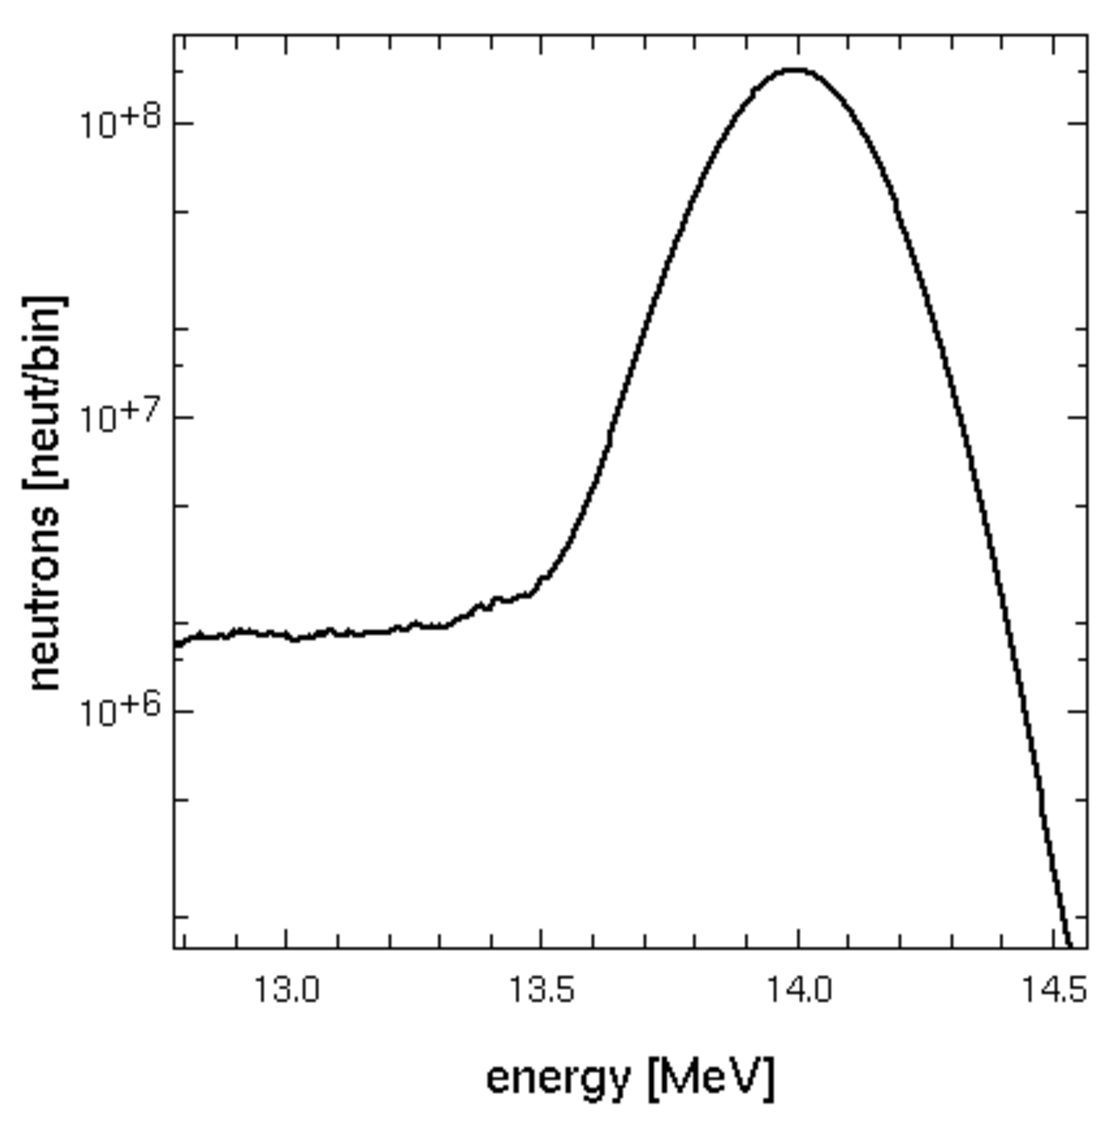
\includegraphics[width=0.8\columnwidth]{neut_spectrum}
\par\end{centering}
\caption{\label{fig:neut_spectrum}simulated DT neutron spectrum. Monte Carlo neutron transport in HYDRA produces detailed neutron spectra. DT neutron spectra show a thermally- and flow-broadened peak centered near 14 MeV. Neutrons scattered by cold DT are also visible here in the band below 13.5 MeV. We compute similar detailed spectra on five diagnostic lines of sight.  We compute less resolved spectra at 1600 locations uniformly distributed on the sphere. }
\end{figure}

Let us first examine the physical processes that shift the centroid
of the primary peak. At its simplest, the peak is located near the
birth energy of DT neutrons. The most obvious shift occurs due to
rigid or bulk translation of the neutron emitting fluid. Heuristically,
we can think that the neutron arrival encodes the neutron birth velocity
and the fluid velocity as $t_{a}=d/\left(v_{0}+v_{fluid}\right)$,
where $v_{0}$ is the birth velocity of DT neutrons, $d$ is the distance
to the detector, and $v_{fluid}$ is the translational velocity of
a fluid element or a continuum undergoing rigid translation. There
is, in addition to this fluid mechanical effect, a thermal contribution
to the peak shift \cite{ballabio_relativistic_tion_1998}. Thermal
velocities of particles are carried into the collision between reactants,
here D and T. The kinetic energy of these particles, relative to the
center-of-mass frame of the collision, promotes the energy that a
neutron carries after the reaction. We can account for these effects
simultaneously by writing the emitted neutron energy in terms of the
energy released by DT reactions, the reactant center-of-mass velocity,
and the reactant kinetic energy. Following {[}ref Munro{]}, we write
\begin{equation}
E_{n}=\frac{m_{\alpha}+Q/2}{m_{D}+m_{T}}Q+\mathbf{p}_{n}\cdot\mathbf{v}_{cm}+\frac{m_{\alpha}+Q}{m_{D}+m_{T}}K\label{eq:peak_loc}
\end{equation}
where $m_{\alpha}$, $m_{D}$, and $m_{T}$ are the alpha, deuteron,
and triton masses. $Q$ is the energy liberated in a DT reaction,
$K$ is the center-of-mass kinetic energy of the reactants, $\mathbf{p_{n}}$
is the neutron momentum, and $\mathbf{v}_{cm}$ is the velocity of
the center of mass of the reactant pair. The first term in equation \ref{eq:peak_loc}
represents the neutron birth energy of a reacting DT pair colliding
with negligible relative velocity, or 14.028 MeV. The second term,
typically about 30 times smaller in NIF ICF implosions, represents
the peak shift due to bulk motion. The last term, another factor of
30 smaller than the second, represents the shift in the peak due to
particle kinetic energy, or for a fluid continuum, the thermal temperature. 

At NIF, a nearly-orthogonal triad of nTOF detectors measures the peak
shift on three lines of sight. The thermal shift is estimated using
measurements of the ion temperature, discussed further below. Thus,
the non-thermal shift can be used as a measure the \textit{neutron-averaged}
bulk velocity along an instrument line of sight. The triad of measurements
gives the resultant vector associated with the center-of-mass or bulk
motion of the entire burning hot spot. At NIF, these velocities have
been observed to range from nearly zero up to 160 km/s with a precision
of less than 30 km/s. Simulations show that these velocities are damaging
to implosions, with 100 km/s velocities resulting in halving of the
neutron yield \cite{spears_mode1_pop_140409}.

The thermal state and the underlying fluid flow also affect the peak
width, with both process affecting the observation more equally than
in the shift case. The width is fundamentally set by Doppler broadening
due to the Maxwellian distribution of ion velocities in the emitting
fluid. However, the peak is additionally broadened by the variance
of the fluid velocity field. We emphasize strongly that the rigid-body
translation or resultant bulk velocity that affects the peak location
does \textit{not} alter the width. Instead, the \textit{spread} in
fluid velocities broadens the peak. We keep with the early work by
Brysk and associate a temperature with the neutron peak width. Here,
we will call this apparent temperature the Brysk temperature, or $T_{Brysk}$.
We follow \cite{murphy_neut_spectrum} and write the apparent temperature
as
\begin{equation}
T_{Brysk}=T_{thermal}+\left(\frac{m_{D}+m_{T}}{k}\right)\sigma_{v}^{2}\label{eq:brysk_width}
\end{equation}
$T_{thermal}$ is the thermodynamic temperature that characterizes
the Maxwellian distribution of ion thermal velocities and $k$ is
Boltzmann's constant. The $\sigma_{v}^{2}$ is the variance of the
emitting plasma velocity field taken along the line of sight of a
detector. We can see that the fluid variance raises the apparent temperature.
Any fluid flow process that increases velocity variance -- rotation,
shear, swirling, turbulence, or simply higher spherical implosion
velocity -- will increase the apparent temperature.

We now examine our 3D simulation to illustrate the connection between
the thermodynamic temperature and the flow field as they contribute
to the neutron spectral peak properties, location and width. We first
consider a two-dimensional histogram of neutron production along a
single line of sight (Figure \ref{fig:tu_distribution}, line of sight 1,
or LOS 1). We have counted the number of neutrons produced at a given
thermal temperature ($T$) and at a given velocity ($u$) along the
line of sight. That is, we build the histogram in $(T,u)$-space.
This histogram is both temporally and spatially integrated. We have
removed production time- and length-scales from the problem and discussion. 

\begin{figure*}[h]
\begin{centering}
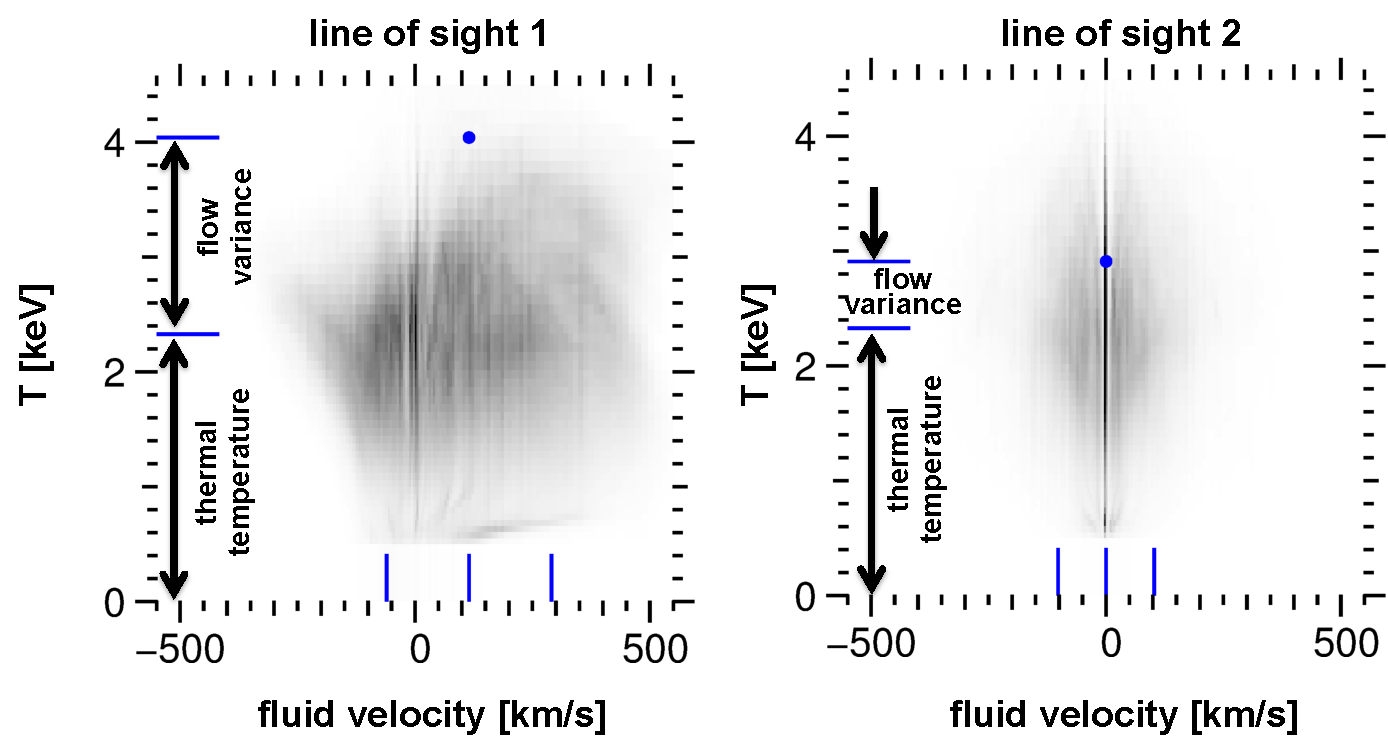
\includegraphics[width=0.8\paperwidth]{tudist}
\par\end{centering}
\caption{\label{fig:tu_distribution}neutron production distributions in temperature and fluid velocity space, or (T,u)-space, for two lines of sight (LOS). We use the total neutron production at each location in (T,u)-space (temporally and spatially integrated) to illustrate the effects of temperature and flow along a line of sight on the peak features. In each panel, the blue tics on the velocity axis indicate the mean (central tic) and variance of the velocity distribution. The tics on the temperature axis indicate the neutron-averaged thermal temperature (lower tic) and the apparent temperature extracted from the spectral peak width. The blue dot indicates the isolated (T,u) conditions that produce a spectrum indistinguishable from that produced by the distributed (grey scale) source. Importantly, the LOS 1 spectrum has large flow variance that greatly raises the apparent temperature above the thermal. The LOS 2 spectrum has a narrower velocity distribution and a temperature closer to thermal. The difference in apparent temperature from LOS to LOS in a measure of the anisotropy of the underlying flow distribution. The associated spectra are included in Figure \ref{fig:los_spectra}.}
\end{figure*}

The LOS 1 $(T,u)$ distribution in Figure \ref{fig:tu_distribution} gives
the spectrum labeled LOS 1 in Figure \ref{fig:los_spectra}. The spectral
peak is shifted slightly by thermal motion, but greatly by the more
than 100 km/s neutron-averaged velocity (indicated by the central
blue tic on the velocity axis). The neutron-averaged velocity does
not affect the width. 

The velocity variance, $\sigma_{v}^{2}$, however, increases the width
substantially beyond the purely thermal broadening (we have indicated
the velocity variance by the leftmost and rightmost blue tics on the
velocity axis). To further clarify the relationship between thermal
temperature and flow, we compare the spectrum produced by the $(T,u)$
distribution along LOS 1 (shown in black in Figure \ref{fig:los_spectra})
with the spectrum produced by a plasma in the localized state denoted
by the blue point in Figure \ref{fig:tu_distribution} on LOS 1. The localized
state has a neutron-averaged velocity equal to that of the distributed
plasma, by crucially, it has no flow variance. Further, the localized
plasma has a thermal temperature of 4 keV. In fact, the spectrum associated
with the gray distribution and that associated with the blue point
are experimentally indistinguishable. Specifically, they have identical
peak widths and peak locations. Thus, a plasma with a 2.4 keV thermal
temperature and flow standard deviation of just over 150 km/s produces
the same peak width as a plasma with no flow variance, but a thermal
temperature of 4 keV. On a single line of sight, we have no way to
determine whether the width is purely thermal or has instead been
augmented by flow effects.

\begin{figure}[h]
\begin{centering}
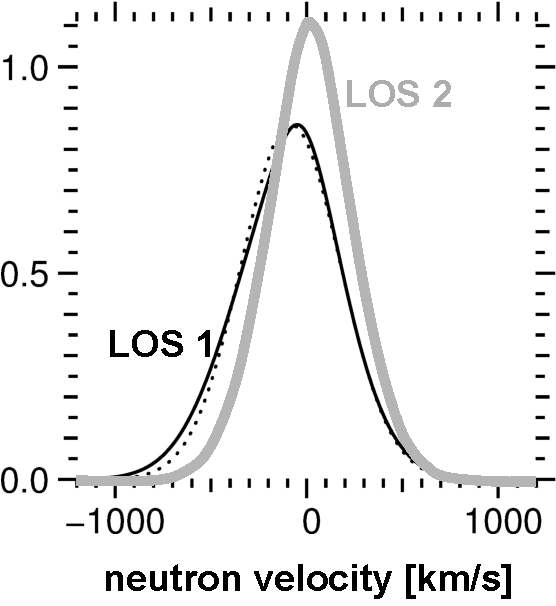
\includegraphics[width=0.8\columnwidth]{los_spectra}
\par\end{centering}
\caption{\label{fig:los_spectra}spectra from the (T,u) distributions in Figure \ref{fig:tu_distribution}. The LOS 1 spectrum is broadened by flow mor than the LOS 2 spectrum. The apparent temperature measure in an experiment would be large for LOS 1 than LOS2.  For comparison, the dotted spectrum is a symmetric Gaussian. Flow effects have also introduced changes in spectral moments beyond the second, including potentially measurable skewness and kurtosis.}
\end{figure}

We can repeat the analysis of the $(T,u)$ distribution and associated
spectrum for a different line of sight which we call LOS 2 (see again
Figure \ref{fig:tu_distribution} and Figure \ref{fig:los_spectra}). On LOS 2,
we see zero neutron-averaged velocity and only 75 km/s of standard
deviation. Consequently, the peak is only slightly upshifted by thermal
effect. The width is narrower on LOS 2 than LOS 1 owing to the much
smaller $\sigma_{v}$ on LOS 2.

We make a key observation when comparing the two lines of sight. While
the thermal temperature is the same for both lines of sight -- there
is, after all, only one plasma producing the neutron signal -- the
flow variance, $\sigma_{v}^{2}$, varies with line of sight due to
the low mode asymmetry of the problem. This asymmetry produces peak
widths that also vary with line of sight. Interpreting the width as
an apparent temperature, we find that $T_{Brysk}$ varies with angle.
The angular $T_{Brysk}$ distribution, produced by the constant thermal
temperature combined with the varying second moment of the velocity
field, must necessarily have a mode 2 distribution, $Y_{2m}$ in spherical
harmonics. 

Our simulation shows the required mode 2 temperature distribution
(see Figure \ref{fig:tion_map}). We record the escaping neutron spectrum
at 1600 locations evenly distributed, then find the apparent temperature
associated with the spectral peak width. This simulated implosion,
which has a thermal temperature of 2.2 keV, shows apparent temperatures
that range from 2.9 keV to 4.0 keV. The major axis of the ellipsoidal
temperature distribution is aligned with the imposed mode-1 asymmetry.
The hot spot flow contains a jet that produces large $\sigma_{v}$
in the direction of the imbalance and small $\sigma_{v}$ in the plane
orthogonal to the imbalance. 

\begin{figure}[h]
\begin{centering}
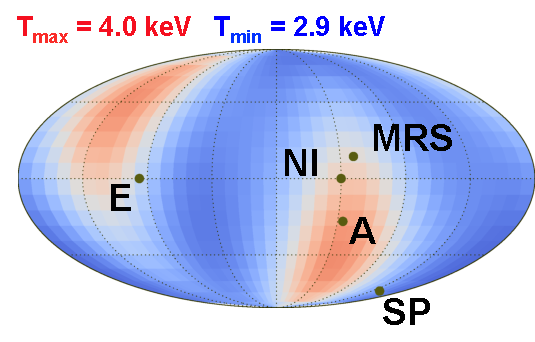
\includegraphics[width=0.8\columnwidth]{tion_map}
\par\end{centering}

\caption{\label{fig:tion_map}projection of the spherical map of apparent ion temperature. We compute the apparent temperature (width of the simulated spectral peak) at 1600 locations over the sphere. The map shows the expected $l=2$ distribution with extremal temperatures of 2.9 keV and 4.0 keV. We also indicate the locations of the 3 nTOF spectrometers (A, E, and SP), the neutron imager time-of-flight spectrometer (NI), and the magnetic recoil spectrometer (MRS). Due to the coverage provided by this array, the spectrometer suite typically captures only half of the total temperature range, in this simulated case 3.0 keV to 3.6 keV.}
\end{figure}

Similar temperature variation can, in principle, occur for any asymmetric
flow producing a velocity field with a variance that depends on angle.
For the purposes of interpreting experimental data we highlight two
ideas. First, the lowest observed temperature is closest to the thermal
temperature. We cannot know what the true thermal temperature is,
but it is certainly no higher than the minimum observation. In our
3D simulation, the lowest possible temperature we could measure (the
direction with minimum variance) would be 2.9 keV, a full 700 eV above
the thermal temperature, but much closer than the 1.8 keV higher maximum.
Second, we emphasize that the difference in temperature with angle
is a measure of residual flow asymmetry in the hot spot. Our heavily
perturbed 3D simulation has a peak-to-valley variation of 1.1 keV.
However, in experiments, we can only measure apparent temperature
on lines of sight where we have spectrometers -- the 3 nTOFs, the
magnetic recoil spectrometer (MRS) \cite{frenje_mrs_dsr,gatujohnson_mrs_velocity_2013},
and the neutron imager time-of-flight detector (NITOF). We show in
Figure \ref{fig:tion_map} the locations of the diagnostics. At these
diagnostic locations, we find a maximum temperature at the specA detector
of 3.56 keV and a minimum at the specSP detector of 2.96 keV. The
observed peak-to-valley apparent temperature difference is only 600
eV, or 54\% of the total variation. In fact, Monte Carlo statistical
analysis shows that this diagnostic array captures only about 50 percent
of the total temperature variation for most temperature distributions.
We should therefore consider measured temperature differences of several
hundreds of eV to indicate appreciable flow asymmetry in the neutron-emitting
hot spot.

\section{\label{sec:experiment}Some comparisons with experiments}

Cryogenic, layered DT implosions on the NIF have generated a collection
of data against which to compare the expectations we have developed
by examining detailed simulated diagnostic output. Some trends in
the data match well our new expectations, including X-ray images and
differences in neutron-based temperature. In contrast, temperature
differences measured using different reactions, DT vs DD, show trends
that are at odds with our simulations and theoretical expectations.

\subsection{\label{sec:sig_asym}signatures of implosion asymmetry}

We now look at the NIF data from recent layered implosions where high-quality
temperature measurements are available from the nTOF detectors. We
use the difference in temperature among diagnostic lines of sight
to estimate the residual flow velocity in implosions. Writing equation \ref{eq:brysk_width}
for the lines of sight with extremal apparent temperature (principle
axes of the velocity variance), we find 

\begin{equation}
T_{max}=T_{thermal}+\left(\frac{m_{D}+m_{T}}{k}\right)\sigma_{v,max}^{2}\label{eq:Tmax}
\end{equation}

\begin{equation}
T_{min}=T_{thermal}+\left(\frac{m_{D}+m_{T}}{k}\right)\sigma_{v,min}^{2}\label{eq:Tmin}
\end{equation}

\begin{equation}
\sigma_{l}\equiv\sqrt{\sigma_{v,max}^{2}-\sigma_{v,max}^{2}}=\sqrt{\frac{k\left(T_{max}-T_{min}\right)}{m_{D}+m_{T}}}\label{eq:observed_spread}
\end{equation}

We derive an lower bound of the residual velocity spread, $\sigma_{l}$,
using the observed maximum and minimum temperatures. In Figure \ref{fig:residual_velocity}
we plot $\sigma_{l}$ $ $ against the maximum temperature difference
measured by the detectors ($T_{max}-T_{min}$). The square root relationship
of equation \ref{eq:observed_spread} is shown in black in the figure. We show
in green and in red the results from a slightly asymmetric 2D simulation
and the very asymmetric 3D simulation. The blue points are the observed
temperature differences for NIF implosions projected onto the black
curve. The temperature differences range from 150 to almost 600 eV,
suggesting that $\sigma_{l}$ ranges from quite small, 70 km/s, to
very large, almost 150 km/s. The largest observed temperature differences
are similar to our heavily perturbed 3D simulation. Of further interest,
we find some correspondence between x-ray image asymmetry and the
observed temperature difference. For example, we consider the shot
N140311, shown in magenta in Figure \ref{fig:residual_velocity}. This temperature
difference indicates a flow asymmetry approaching the levels of the
3D simulation. In Figure \ref{fig:xray_comparison_expt_sim}, we compare
the experimental X-ray image from N140311 with the simulated image
from our 3D simulation. The simulation was not meant to replicate
the conditions of N140311. Nevertheless, the similarity in the x-ray
image distortion and the similarity in the neutron temperature asymmetry
is encouraging.

\begin{figure}[h]
\begin{centering}
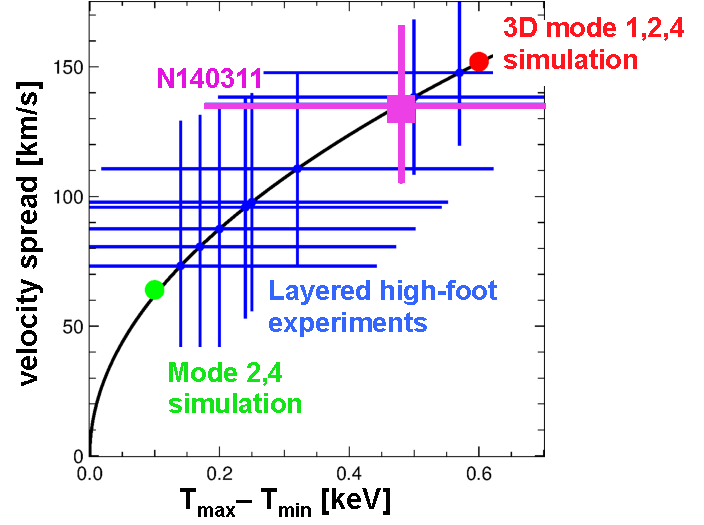
\includegraphics[width=0.8\columnwidth]{residual_velocity}
\par\end{centering}

\caption{\label{fig:residual_velocity} fluid velocity standard deviation versus apparent temperature difference. We plot the expected trend of velocity spread versus maximum difference between the nTOF apparent temperature measurements. We show in blue the measured temperature differences experimental implosions at NIF. We project the values into velocity spread using equation \ref{eq:observed_spread} We highlight the magenta point indicating experiment N140311 (see Figure \ref{fig:xray_comparison_expt_sim}). We also show a lightly perturbed 2D simulated implosion (green) and the heavily perturbed 3D simulation (red). The experiments show a large range of inferred residual hot spot velocity with several experiments approaching 150 $km/s$.}
\end{figure}

\begin{figure}[h]
\begin{centering}
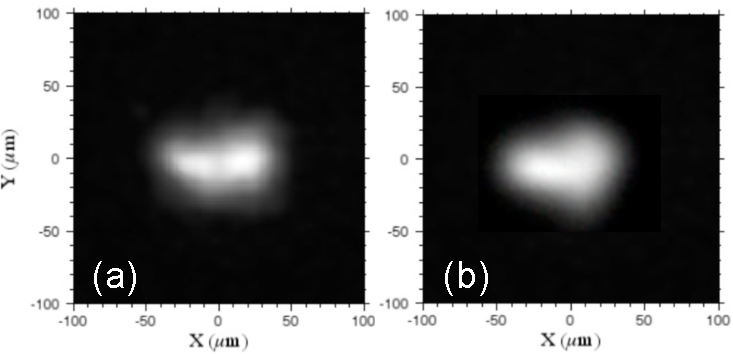
\includegraphics[width=0.8\columnwidth]{xray_comparison_expt_sim}
\par\end{centering}

\caption{\label{fig:xray_comparison_expt_sim}comparison of experiment N140311 with the 3D simulation. We compare the level of asymmetry seen in the experimental X-ray image (a) with the simulated image (b). While the simulation is not intended to represent exactly the experiment, the degree of asymmetry in the images is similar.  Furthermore, the simulated hot spot flow spread lies within the error bar for the experimental inference. See Figure \ref{fig:residual_velocity}. }
\end{figure}

\subsection{\label{sec:dd_dt_expts}DD and DT neutron yield trends for further investigation.  }

We can apply the theory for flow impact on apparent temperature equally
well to the neutron peak produced by DT or DD reactions. The only
change to equation \ref{eq:brysk_width} upon switching reactions is in the
total mass of the reactants; for DD we use $(m_{D}+m_{D})$ in place
of $(m_{D}+m_{T})$. The mass change alters the weight of the contribution
of the non-thermal motion to the width and associated apparent temperature,
$T_{Brysk}$. So, we use equation \ref{eq:Tmax} and equation \ref{eq:Tmin}
for both DD and DT to compute the line-of-sight temperature difference
$\Delta T=T_{max}-T_{min}$. We find
\begin{equation}
\frac{\Delta T_{DT}}{\Delta T_{DD}}=\frac{T_{max,DT}-T_{min,DT}}{T_{max,DD}-T_{min,DD}}=\frac{m_{D}+m_{T}}{m_{D}+m_{D}}=\frac{5}{4}
\label{eq:dt_dd_ratio}
\end{equation}
This simple result suggests we should find temperature variation with
line of sight, that is 25\% greater for DT than for DD. In fact, we
find this ratio for our perturbed 3D simulation to be almost exactly
$\frac{5}{4}$ (see Figure \ref{fig:tion_dd_dt}). However, we also show
in Figure \ref{fig:tion_dd_dt} the experimental data -- it does not agree.
The experiments show that the the $\Delta T_{DD}$ is almost always
larger than $\Delta T_{DT}$. Moreover, the experimental DD and DT
quantities appear to be independent of one another. This surprising
relationship suggests we have more to learn about interpreting the
spectral peak properties. We would like to hypothesize that greater
scattering by DD neutrons as compared to DT neutrons sets up potential
screening issues. We imagine that the heavy scattering of DD neutrons
means that the detected unscattered DD peak neutrons emanate from
a more localized (e.g., nearer) region of the hot spot. The lightly
scattered DT neutrons, by contrast, issue more nearly from the entire
hot spot. This would set up a biasing such that DD and DT neturons
are really sampling different material regions, thereby breaking equation \ref{eq:dt_dd_ratio}
which assumes the neutron signals sample the same flows. Yet, our
3D simulation and associated particle transport package are aware
of this very process. Still, the simulation respects equation \ref{eq:dt_dd_ratio}.
We have more to learn, and further numerical investigations into the
detailed locations of particular particle birth and scattering events
for a variety of hot spot and fuel conformations may shed some light. 

\begin{figure}[h]
\begin{centering}
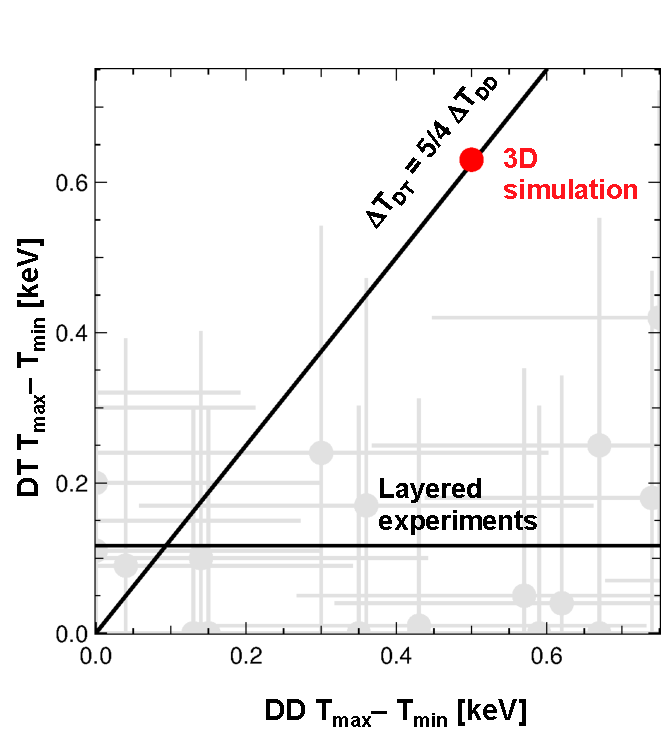
\includegraphics[width=0.8\columnwidth]{tion_dd_dt}
\par\end{centering}
\caption{\label{fig:tion_dd_dt}DD
comparison of line-of-sight apparent temperature variation for DD and DT neutrons. We compute the difference between maximum and minimum apparent temperatures for NIF high foot experiments for both DD and DT neutrons (gray points). We show also the expected temperature scaling and the surprising fit to the experimental data. This surprising relationship between DD and DT temperature anisotropy suggests that we are missing ingredients in our understanding of the stagnated fuel assembly.}
\end{figure}

\section{\label{sec:conclusion}Conclusions}

We have demonstrated a new capability for performing 3D simulations
of NIF implosions with multimode drive asymmetry and simultaneous
detailed diagnostic output. Our analysis of the simulated diagnostic
output for both a particular asymmetric 3D implosion provides some
new insight into both X-ray and neutron signatures of asymmetry. We
find that highly time- and space-resolved X-ray images, like those
provided by NIF's DIXI camera, show hot spot features that have spatial
scale lengths in the range of 10 $\mu m$ and flow features that evolve
on time scales shorter than 30 ps. In contrast to conventional expectations,
the X-ray images show little shape variation with X-ray spectral energy.
When comparing X-ray images to neutron images, however, we find differences.
We attribute these differences to the different emissivities for neutrons
and X-rays, as well as the different electron and ion temperatures
during the early period of X-ray production. Turning to neutron spectral
features, we see that flow in the hot spot, either bulk translation
or internal swirling, alters the neutron peak. The bulk translation
shifts the center energy of the peak. The hot spot flow velocity variance
-- swirl, shear, rotation -- increases the peak width along a given
line of sight. This broadening due to non-thermal motion is indistinguishable
from that due to thermal motion. We can examine this broadening, or
increase in apparent temperature, from multiple lines of sight to
derive a lower bound on the residual velocity variance in the hot
spot. We perform this analysis on NIF experimental data. The results
show flow velocities ranging from nearly negligible to quite high,
with the highest levels being comparable to those seen in our highly
perturbed simulation. The implication is that the neutron spectral
data support the inference from the X-ray data that the implosions
are often appreciably perturbed. Further, the neutron data can provide
a quantitative measure of the asymmetry-induced residual flow. Not
all data follows our theory and simulations. The most striking discrepancy
comes in the relationship between the DT and DD apparent temperature
asymmetry. Not only do the temperature asymmetries appear larger in
DD than in DT, in direct opposition to our new expectations, but the
DD and DT asymmetries appear to be independent of one another. Overall,
this exercise has provided us with a better informed set of expectations
for experimental data from asymmetric implosions. Some of our new
expectations are supported. Some are not, and these provide an opportunity
for further insight as we strive to reconcile the discrepancies.

\begin{acknowledgments}
Prepared by LLNL under Contract DE-AC52-07NA27344.
\end{acknowledgments}

\bibliographystyle{plain}
\bibliography{/Users/spears9/Files/mypapers/spears_refs}

\end{document}
